\section{Application des TBCs approximées à une Méthode de Décomposition de Domaine}

\indent L'approximation des conditions aux limites transparentes (TBCs) utilisant un polynôme constant sera appliquée dans une Méthode de Décomposition de Domaine (\emph{Domain Decomposition Method} - DDM). On va d'abord décrire le DDM qu'on utilisera ici, et ensuite on décrira et testera l'incorporation des TBCs.

\subsection{The Schwarz Methods}

\indent La description suivante s'appuye sur \cite{Japhet2003}. Les Méthodes de Décomposition de Domaines, comme indique son nom, permettent de décomposer un domaine $\Omega$ en plusieurs subdomaines $\Omega_i$ (superposés ou pas) et de résoudre le problème dans chacun d'eux. Ainsi, il faut trouver des fonctions qui satisfassent la PDE dans chacun des subdomaines et que soient égaux dans les interfaces.

\indent La première DDM développée a été la méthode de Schwarz \cite{Japhet2003,Gander2008}, qui consiste en une méthode itérative : dans le cas d'un problème d'évolution, la solution $u_i^{n,\infty}$, dans chaque pas de temps $t_n$ et chaque subdomaine $\Omega_i$, est calculée comme étant la convergence de la solution obtenue dans chaque itération, $u_i^{n,k}, \ \ k\geq 0$. Il y a deux types de méthodes de Schwarz, en dépendant de la manière avec laquelle las conditions aux interfaces sont construites pour calculer $u_i^{n,k}$.

\indent Dans la méthode de Schwarz additive (\emph{Additive Schwarz Method - ASM}), les conditions aux interfaces sont toujours calculées en utilisant la solution $u_j^{n,k-1}, \ \ j \neq i$ de la dernière itération. Ainsi, dans l'interface entre les domaines $\Omega_i$ et $\Omega_j$, les conditions à l'interface pour le problème $\Omega_i$ s'écrit comme

$$\mathcal{B}_i(u_i^{n,k+1}) = \mathcal{B}_i(u_j^{n,k})$$

\noindent où $\mathcal{B}$ est l'opérateur de la TBC.

\indent En revanche, la méthode de Schwarz multiplicative (\emph{Multiplicative Schwarz Method - MSM}) utilise toujours l'information la plus récente pour le calcul des conditions aux interfaces. Ainsi, dans le cas d'une DDM avec deux subdomains, les TBCs s'écriraient (par exemple) sous la forme

$$\mathcal{B}_1(u_1^{n,k+1}) = \mathcal{B}_1(u_2^{n,k}) \\ \mathcal{B}_2(u_2^{n,k+1}) = \mathcal{B}_2(u_1^{n,k+1})$$

\noindent pour la résolution du problème dans $\Omega_1$ et $\Omega_2$, respectivement. En fait, la MSM a été la forme originale proposée par Schwarz (avec une condition du type Dirichlet, $\mathcal{B_i}(u) = u$)  \cite{Japhet2003,Lions1990}. L'ASM est une modification proposée par \cite{Lions1988}, et qui présente comme principale avantage (notamment quand le nombre de subdomaines augmente) le fait d'être un algorithme naturellement parallèle (et qui peut ainsi être implémenté en utilisant la computation parallèle) \cite{Lions1988}.

\indent Dans le stage, on n'a travaillé qu'avec l'ASM. Par ailleurs, on a toujours considéré une DDM décomposant $\Omega \subset \mathcal{R}$ dans deux subdomaines $\Omega_1$ et $\Omega_2$, non superposants (sauf par un point en commun). La description faite dans ce rapport considère toujours ces hypothèses, mais elle serait équivalente dans le cas de DDMs plus générales.

\indent On veut qu'une DDM présente les propriétés suivantes :

\begin{itemize}
   	\item Il y a une unique solution $\Omega_i$ dans chaque subdomaine $\Omega_i$.
	\item La solution $u_i$ dans chaque subdomaine $\Omega_i$ converge vers $u|_{\Omega_1}$, i.e, la solution $u$ du monodomaine $\Omega$ restreinte à $\Omega_1$
	\item La méthode converge rapidement
\end{itemize}

\indent Selon \cite{Japhet2013}, l'ASM optimale est celle qui utilise les exactes TBCs \eqref{eq:exactTBC} comme conditions aux interfaces : dans ce cas, la méthode converge dans deux itérations, et aucune autre ASM ne peut converger plus rapidement. Néanmoins, comme discuté avant dans ce rapport, la dérivation analytique et l'implémentation numérique des TBCs exactes sont, en général, impraticables, en raison de son caractère non local en temps. Ainsi, on propose ici l'implémentation des TBCs approximées \eqref{eq:appTBCP0} dans la DDM.

\subsection{ASM avec des TBCs approximées pour l'équation de dispersion}

\indent La résolution de l'équation de dispersion avec la Méthode de Schwarz Additive, en utilisant l'approximation des TBCs construite à partir d'un polynôme constant, s'écrit comme

\begin{equation}
    \label{eq:problemDDM1}
    \begin{cases}
        (u_1^{n,k+1})_t + (u_1^{n,k+1})_{xxx} = 0 , \ \ x \in \Omega_1, \ \ t \geq 0\\
        u_1^{n,0} = u_1^{n-1,\infty} , \ \ x \in \Omega_1 \\
        \Upsilon_1^{c_L}(u_1^{n+1,k+1},-L) = 0, \\ 
        \Theta_2^{c_R}(u_1^{n+1,k+1},0) = \Theta_2^{c_R}(u_2^{n,k},0) , \\
        \Theta_3^{c_R}(u_1^{n+1,k+1},0) = \Theta_3^{c_R}(u_2^{n,k},0)
     \end{cases}
\end{equation}

\begin{equation}
    \label{eq:problemDDM2}
    \begin{cases}
        (u_2^{n,k+1})_t + (u_2^{n,k+1})_{xxx} = 0 , \ \ x \in \Omega_2, \ \ t \geq 0\\
        u_2^{n,0} = u_2^{n-1,\infty} , \ \ x \in \Omega_2 \\
        \Theta_1^{c_L}(u_2^{n+1,k+1},0) = \Theta_1^{c_L}(u_1^{n,k},0) \\
        \Upsilon_2^{c_R}(u_2^{n+1,k+1},L) = 0 \\
        \Upsilon_3^{c_R}(u_2^{n+1,k+1},L) = 0
     \end{cases}
\end{equation}

\noindent où $ \Upsilon_i, \ \ i=1,2,3$,  sont les conditions aux limites sur les bords extérieurs (i.e., définies sur $\partial Delta_i \backslash \Gamma$). Ces conditions externes sont indépendantes des conditions à l'interface. On va considérer ici $\Upsilon_1 = \Theta_1^{1.0}$, $\Upsilon_2 = \Theta_2^{0.0}$ and $\Upsilon_3 = \Theta_3^{0.0}$, ce qui donne 

\begin{equation}
\label{eq:externalBCsDDM}
\begin{gathered}
	\Upsilon_1(u,x) = u - u_x + u_{xx} \\
	\Upsilon_2(u,x) = 0 \\
	\Upsilon_3(u,x) = 0
\end{gathered}
\end{equation}

\indent Ce choix a été fait en se basant sur son implémentation simple et sur les bons résultats fournis par les coefficients $c_L = 1.0$ et $c_R = 0.0$ lors de l'approximation de la solution analytique dans $\Omega$ (comme montre le tableau \ref{tab:firstTestsP0}). Néanmoins, cela n'a pas une vraie importance dans l'étude qu'on propose ici, parce qu'on va comparer les résultats de la DDM avec une solution numérique de référence calculée  dans le monodomaine. La seule exigence pour que cet étude soit cohérent est que les conditions aux limites externes pour le calcul de $u^{ref}$ soient les mêmes $\Upsilon_i, \ \ i=1,2,3$ utilisées dans la DDM.

\indent Ainsi, la solution de référence utilisé dans cet étude est la solution du problème

\begin{equation}
	\label{eq:problemMonodomain}
	\begin{cases}
	u_t + u_{xxx} = 0, \ \ x \in \Omega, \ \ t \in [t_0, t_0+\Delta t] \\
	u(t_0,x) = u^{exact}(t_0,x) , \ \ x \in \Omega \\ 
	\Upsilon_1(u,-L) = 0, \ \ t \in [t_0, t_0+\Delta t] \\
	\Upsilon_2(u,L) = 0, \ \ t \in [t_0, t_0+\Delta t] \\
	\Upsilon_3(u,L) = 0, \ \ t \in [t_0, t_0+\Delta t]
	\end{cases}
\end{equation}


\paragraph{Remarques sur la notation}

\indent Toujours en considérant les objectifs de ce travail, on remarque qu'on va comparer les solutions calculées seulement dans un pas de temps. Cela est nécessaire pour que l'erreur due à la DDM soit étudiée séparément (sans influence, para exemple, de l'erreur accumulée au long des pas de temps, due à la discrétisation temporale).

\indent Par conséquent, on peut alléger la notation. À parti d'ici jusqu'à la fin de ce rapport, on notera par $u_j^i$ la solution du DDM, où $i$ indique le subdomaine $\Omega_i$ (ou, dans le cas de la solution de référence, $i=ref$, et à convergence de la méthode, $i=*$) et $j$ indique la position spatiale discrète. Dans les cas où le processus itérative doit être considéré, on ajoutera le superindice $k$ pour indique l'itération.

\indent En ce qui concerne la discrétisation spatiale, le monodomain $\Omega$ sera divisé en $2N+1$ points distribués de façon homogène, numérotés de $0$ jusqu'à $2N$. Dans les descriptions suivantes, on va considérer toujours que les deux subdomaines $\Omega_1$ et $\Omega_2$ ont le même nombre de points, respectivement  $x_0,...,x_N$ et $x_N,...,x_{2N}$. Le point à l'interface, $x_N$, est commun aux deux subdomains, ayant des solutions différentes dans chacun d'eux : $u_N^1$ et $u_N^2$. Évidemment, on espère que, à convergence, $u_N^1 = u_N^2 = u_N^*$.


\subsection{Discrétisation du problème et erreur dans la solution convergée}

\indent Lors de l'application de TBCs approximés dans une ASM, on doit assurer que la solution convergée $u^*$ satisfait la même équation discrète que la solution $u^{ref}$ du problème dans le monodomaine. Dans les paragraphes suivants, on va montrer que cette propriété n'est pas vérifiée par la méthode  \eqref{eq:problemDDM1} - \eqref{eq:problemDDM2} proposée ici, et, en se basant sur cette démonstration, on proposera des corrections pour ce problème.

\indent Pour les points intérieurs de chacun des domaines, on considérera une discrétisation spatiale de seconde ordre pour l'équation \eqref{eq:DKdV} :

\begin{equation}
    \label{eq:FDdiscretization}
    \frac{u_j^i - \alpha_j^i}{\Delta t} + \frac{-\frac{1}{2}u_{j-2}^i + u_{j-1}^i - u_{j+1}^i + \frac{1}{2}u_{j+2}^i }{\Delta x ^3} = 0
\end{equation}

\noindent ce qui est valide pour $j=2,...,N-2$ dans le cas $i=1$; pour $j=N+2,...,2N-2$ dans le cas $i=2$; et pour $j=2,...,2N-2$ dans le cas $i=ref$. Dans \eqref{eq:FDdiscretization}, $\alpha_j^i$ est une donnée (par exemple, la solution convergé du pas de temps précédent).

\indent Pour les points proches aux bords, on utilise une discrétisation décentrée ou les TBCs appropriées. En fait, en considérant qu'une TBC est écrite pour le bord à gauche et deux pour le bord à droite, on doit imposer une discrétisation décentrée seulement pour le deuxième point le plus proche du bord à gauche. Par exemple, pour le point $x_1$ : 

\begin{equation}
    \label{eq:uncenteredFDdiscretization0}
    \frac{u_{1}^2 - \alpha_{1}^2}{\Delta t} + \frac{-\frac{5}{2}u_{1}^2 + 9u_{2}^2 - 12 u_{3}^2 + 7\frac{1}{2}u_{4}^2 -\frac{3}{2}u_{5}^2}{\Delta x ^3} = 0
\end{equation}

\noindent et de façon similaire pour les autres points proches des bords.

\indent Pour résoudre le problème dans $\Omega_1$, two interface boundary conditions are imposed (corresponding to $\Theta_2$ and $\Theta_3$) to the discrete equations for the points $x_{N-1}$ and $x_N$ : 

\begin{equation}
	\begin{aligned}
    \label{eq:TBCsIterOmega1A}
    && 				&\Theta_2^{c_R}(u_N^1) = \Theta_2^{c_R}(u_N^2) \implies \\ 
    && \implies & u_N^1 - c_R^2 \frac{u_N^1 - 2u_{N-1}^1 + u_{N-2}^1}{\Delta x^2} = u_N^2 - c_R^2 \frac{u_N^2 - 2u_{N+1}^2 + u_{N+2}^2}{\Delta x^2} 
    \end{aligned}
\end{equation}

\begin{equation}
	\begin{aligned}
    \label{eq:TBCsIterOmega1B}
    && 			   & \Theta_3^{c_R}(u_N^1) = \Theta_3^{c_R}(u_N^2) \implies \\
    && \implies & \frac{u_N^1 - u_{N-1}^1}{\Delta x} + c_R \frac{u_N^1 - 2u_{N-1}^1 + u_{N-2}^1}{\Delta x^2} = \frac{u_{N+1}^2 - u_{N}^2}{\Delta x} + c_R \frac{u_N^2 - 2u_{N+1}^2 + u_{N+2}^2}{\Delta x^2}
    \end{aligned}
\end{equation}

\indent En revanche, pour résoudre le problème dans $\Omega_2$, seulement une condition à l'interface est utilisée (correspondant à $\Theta_1$), étant imposée pour le point $x_N$ : 

\begin{equation}
	\begin{aligned}
    \label{eq:TBCsIterOmega2}
    && 				&\Theta_1^{c_L}(u_N^2) = \Theta_1^{c_L}(u_N^1) \implies \\ 
    && \implies & u_N^2 - c_L \frac{u_{N+1}^2 - u_{N}^2}{\Delta x} + c_L^2 \frac{u_N^2 - 2u_{N+1}^2 + u_{N+2}^2}{\Delta x^2}  =\\
    && 				& u_N^1 - c_L \frac{u_{N}^1 - u_{N-1}^1}{\Delta x} + c_L^2 \frac{u_N^1 - 2u_{N-1}^1 + u_{N-2}^1}{\Delta x^2}
    \end{aligned}
\end{equation}

\indent À convergence, les expressions \eqref{eq:TBCsIterOmega1A} jusqu'à \eqref{eq:TBCsIterOmega2} donnent respectivement 


\begin{equation*}
    \label{eq:TBCsCVOmega1A}
\begin{aligned}
   \bullet \qquad && 			    &u_N^* - c_R^2 \frac{u_N^* - 2u_{N-1}^* + u_{N-2}^*}{\Delta x^2} = u_N^* - c_R^2 \frac{u_N^* - 2u_{N+1}^* + u_{N+2}^*}{\Delta x^2} \implies  \\
    && \implies & 2c_R^2 \frac{-\frac{1}{2}u_{N-2}^* + u_{N-1}^* - u_{N+1}^* + \frac{1}{2}u_{N+2}^* }{\Delta x^2} = 0
    \end{aligned}
    \end{equation*}
    
\begin{equation*}
    \label{eq:TBCsCVOmega1B}
\begin{aligned}
    \bullet \qquad &&             &\frac{u_N^* - u_{N-1}^*}{\Delta x} + c_R \frac{u_N^* - 2u_{N-1}^* + u_{N-2}^*}{\Delta x^2} = \\
    && 			   &\frac{u_{N+1}^* - u_{N}^*}{\Delta x} + c_R \frac{u_N^* - 2u_{N+1}^* + u_{N+2}^*}{\Delta x^2} \implies \\
    && \implies & -\frac{u_{N-1}^* - 2 u_{N}^* + u_{N+1}^*}{\Delta x} - 2c_R\frac{-\frac{1}{2}u_{N-2}^* + u_{N-1}^* - u_{N+1}^* + \frac{1}{2}u_{N+2}^* }{\Delta x^2} = 0 
\end{aligned}
\end{equation*}

\begin{equation*}
    \label{eq:TBCsCVOmega2}
\begin{aligned}
   \bullet \qquad && 					&	 u_N^* -  c_L\frac{u_{N+1}^* - u_{N}^*}{\Delta x} + c_L^2 \frac{u_{N}^* - 2u_{N+1}^* + u_{N+2}^*}{\Delta x^2} =  \\
   && 					& u_N^* -  c_L\frac{u_{N}^* - u_{N-1}^*}{\Delta x} + c_L^2 \frac{u_{N}^* - 2u_{N-1}^* + u_{N-2}^*}{\Delta x^2} \implies \\
	&&  \implies	    & -c_L\frac{u_{N-1}^* - 2 u_{N}^* + u_{N+1}^*}{\Delta x} + 2c_L^2\frac{-\frac{1}{2}u_{N-2}^* + u_{N-1}^* - u_{N+1}^* + \frac{1}{2}u_{N+2}^* }{\Delta x^2} = 0 
\end{aligned}
\end{equation*}

\indent Alors, on peut observer que la solution convergée de la DDM ne satisfait pas la même équation discrète que la solution de référence dans les points $x_{N-1}, x_N \in \Omega_1$, et dans $x_N\in \Omega_2$. Dans tous les autres points les équations satisfaites sont identiques, à l'exception du point $x_{N_1} \in \Omega_2$, comme détaillé dans la remarque suivante :

\paragraph{Remarque : modification de la solution de référence :}

\indent Même si la DDM fournissait une solution compatible avec celle du problème dans le monodomain (ce qu'on va imposer avec des corrections proposées dans la suite de ce rapport), la solution de la DDM ne convergerait exactement vers $u^{ref}$, pour une raison qui ne dépendent pas de l'expression des IBCs, mais si du fait qu'on écrit deux IBCs pour le bord à gauche et une pour le droit. Comme on utilise une discrétisation centrée pour la troisième dérivative dans l'espace (ce qui demande un stencil de deux points de chaque côté du point au milieu), il faut écrire une discrétisation décentrée pour le point $x_{N+1}$  lors de la résolution du problème dans $\Omega_2$. Ainsi, ce point ne satisfait pas la même équation discrète que dans le problème de référence. Afin d'éviter cette incompatibilité et de nous permettre de bien étudier le comportement de la DDM, on va modifier la discrétisation du point  $x_{N+1}$ dans problème du monodomain, en utilisant la même discrétisation décentrée de seconde ordre :

\begin{equation*}
    \label{eq:uncenteredFDdiscretizationN}
    \frac{u_{N+1}^2 - \alpha_{N+1}^2}{\Delta t} + \frac{-\frac{5}{2}u_{N+1}^2 + 9u_{N+2}^2 - 12 u_{N+3}^2 + 7\frac{1}{2}u_{N+4}^2 -\frac{3}{2}u_{N+1}^2}{\Delta x ^3} = 0
\end{equation*}

\indent Étant faite cette remarque, la figure \ref{fig:discretizations} résume les discrétisations imposées pour chaque point dans les problèmes du monodomain et de la DDM, selon da description faite ci-dessus :

\indent

\begingroup
\tikzstyle{label} =[above,font=\tiny]
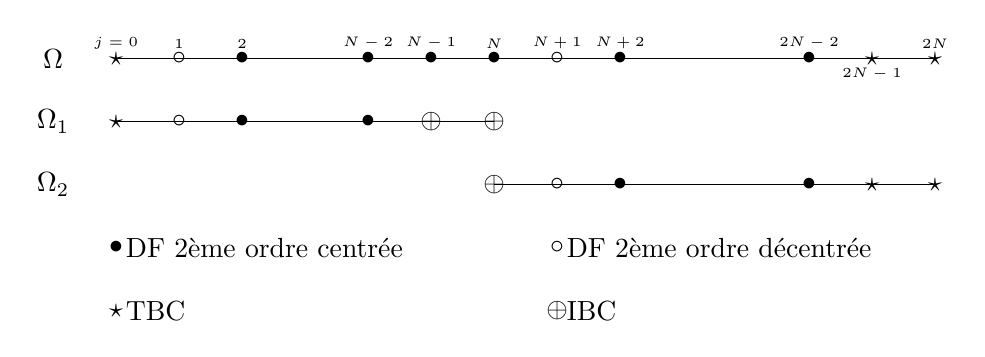
\begin{tikzpicture}[scale = .8]
	\coordinate (Alabel) at (-1,3);
	\coordinate (Aa) at (0,3);
	\coordinate (Ab) at (1,3);
	\coordinate (Ac) at (2,3);
	\coordinate (Ad) at (4,3);	
	\coordinate (Ae) at (5,3);	
	\coordinate (Af) at (6,3);	
	\coordinate (Ag) at (7,3);	
	\coordinate (Ah) at (8,3);	
	\coordinate (Ai) at (11,3);
	\coordinate (Aj) at (12,3);
	\coordinate (Ak) at (13,3);
	
	\draw (Aa) -- (Ak);
	\draw (Alabel) node {$\Omega$}; 
	\draw (Aa) node[label] {$j=0$};
	\draw (Ab) node[label] {$1$};
	\draw (Ac) node[label] {$2$};
	\draw (Ad) node[label] {$N-2$};
	\draw (Ae) node[label] {$N-1$};
	\draw (Af) node[label] {$N$};
	\draw (Ag) node[label] {$N+1$};
	\draw (Ah) node[label] {$N+2$};
	\draw (Ai) node[label] {$2N-2$};
	\draw (Aj) node[below,font=\tiny] {$2N-1$};
	\draw (Ak) node[label] {$2N$};
		
	\draw (Aa) node {$\star$};
	\draw (Ab) node {$\circ$};
	\draw (Aj) node {$\star$};
	\draw (Ak) node {$\star$};
	
	\draw (Ac) node{$\bullet$};
	\draw (Ad) node {$\bullet$};
	\draw (Ae) node {$\bullet$};
	\draw (Af) node{$\bullet$};	
	\draw (Ag) node{$\circ$};
	\draw (Ah) node {$\bullet$};
	\draw (Ai) node {$\bullet$};


	\coordinate (Blabel) at (-1,2);	
	\coordinate (Ba) at (0,2);
	\coordinate (Bb) at (1,2);
	\coordinate (Bc) at (2,2);
	\coordinate (Bd) at (4,2);	
	\coordinate (Be) at (5,2);	
	\coordinate (Bf) at (6,2);	

	\draw (Ba) -- (Bf); 
	
	\draw (Blabel) node {$\Omega_1$}; 
	\draw (Ba) node {$\star$};
	\draw (Bb) node {$\circ$};
	
	\draw (Bc) node {$\bullet$};
	\draw (Bd) node {$\bullet$};
	
	\draw (Be) node {$\oplus$};
	\draw (Bf) node {$\oplus$};	
	
	\coordinate (Clabel) at (-1,1);	
	\coordinate (Cf) at (6,1);	
	\coordinate (Cg) at (7,1);	
	\coordinate (Ch) at (8,1);	
	\coordinate (Ci) at (11,1);
	\coordinate (Cj) at (12,1);
	\coordinate (Ck) at (13,1);
		
	\draw (Cf) -- (Ck); 
	\draw (Clabel) node {$\Omega_2$}; 
	\draw (Cf) node{$\oplus$};
	\draw (Cg) node{$\circ$};
	\draw (Ch) node{$\bullet$};	
	\draw (Ci) node{$\bullet$};	
	\draw (Cj) node {$\star$};
	\draw (Ck) node{$\star$};
	
	%% Legend
	\draw (0,0) node {$\bullet$} node[right] {DF 2ème ordre centrée};
	\draw (7,0) node {$\circ$} node[right] {DF 2ème ordre décentrée};
	\draw (0,-1) node {$\star$} node[right] {TBC};
    \draw (7,-1) node {$\oplus$} node[right] {IBC};
	
\end{tikzpicture}
\captionof{figure}{Schéma indiquanla discrétisation spatiale imposée pour chaque point du monodomaine et des subdomaines de la DDM \label{fig:discretizations}}
\endgroup


\subsubsection{Numerical verification of the error}

\indent Le problème \eqref{eq:problemDDM1} - \eqref{eq:problemDDM2} a été résolu jusqu'à convergence avec cinq discrétisations spatiales uniformes différentes, au long d'un pas de temps (dans l'intervale $[0,\Delta t]$). Dans chaque cas, la solution de référence $u^{ref}$ était la solution du problème du monodomain \eqref{eq:problemMonodomain}, résolu avec la même taille de maille. Deux erreurs ont été calculées :

\begin{equation*}
	e^{N,*} = |u^{ref}_N - u^{*}_N|
\end{equation*}

\begin{equation}
	\label{eq:errorDDM}
	e^{\Omega,*} = ||u^{ref}_N - u^{*}_N||_2 = \sqrt{\Delta x \left[ \sum_{j=0}^N{(u^{ref}_j - u^{1,\infty}_j)^2 } + \sum_{j=N}^{2N}{(u^{ref}_j - u^{2,\infty}_j)^2 } \right] }
\end{equation}

\noindent correspondant respectivement à l'erreur sur l'interface et à l'erreur dans tout le domain.

\indent On s'intéresse au comportement de ces erreurs en fonction de la taille de maille. Comme montré la figure \ref{fig:orderVerification}, on vérifie que la DDM proposée par nous produit une erreur d'ordre $O(\Delta x)$  :

\begingroup
\begin{center}
	\includegraphics[scale=.5]{figures/convergenceVerificationCorrectN.png}
	\captionof{figure}{Vérification numérique de l'ordre de convergence de l'erreur due à la DDM \label{fig:orderVerification}}
\end{center}
\endgroup

\subsubsection{Corrections pour les TBCs approximées}

\indent On va formuler des modifications pour les TBCs utilisées dans l'ASM afin d'annuler ces erreurs :

\begin{equation*}
    \begin{gathered}
        \Theta_1^{c_L}(u_2^{n+1,k+1}) + \theta_1 = \Theta_1^{c_L}(u_1^{n,k}) + \theta_1' \\
        \Theta_2^{c_R}(u_1^{n+1,k+1}) + \theta_2 = \Theta_2^{c_R}(u_2^{n,k}) + \theta_2' \\
        \Theta_3^{c_R}(u_1^{n+1,k+1}) + \theta_3 = \Theta_3^{c_R}(u_2^{n,k}) + \theta_3'
    \end{gathered}
\end{equation*}

\noindent avec $\theta_i, \theta_i'$  donnés par 

\begin{gather*}
    \theta_1 = \Delta x c_L \frac{u_{N+1}^2 - 2u_{N}^2 + u_{N-1}^1}{\Delta x^2} + c_L^2\frac{\Delta x}{\Delta t} \left( u_{N}^2 - \alpha_{N}^2 \right)\\
    \theta_1' = - c_L^2\frac{\Delta x}{\Delta t} \left( u_{N}^1 - \alpha_{N}^1 \right)
\end{gather*}

\begin{equation*}
\begin{gathered}
    \theta_2 = \frac{\Delta x}{\Delta t} c_R^2 (u_N^1 - \alpha_N^1) \\
    \theta_2' = -\frac{\Delta x}{\Delta t} c_R^2 (u_N^2 - \alpha_N^2)
\end{gathered}
\end{equation*}

\begin{equation*}
\begin{gathered}
    \theta_3 = 2\frac{\Delta x}{\Delta t} \left[-\Delta x(u_{N-1}^1 - \alpha_{N-1}^1) - c_R (u_N^1 - \alpha_N^1) \right] + \Delta x \frac{u_{N-3}^1 - 2u_{N-2}^1 + u_{N-1}^1}{\Delta x^2} \\
    \theta_3' = 0
\end{gathered}
\end{equation*}

\indent En fait, on a, dans la convergence de la première condition à l'interface :

\begin{equation*}
\label{eq:modifiedTBC1}
\begin{aligned}
&& &    \Theta_1^{c_L}(u_N^*) + \theta_1 = \Theta_1^{c_L}(u_N^*) + \theta_1' \\
&& \implies &    u_N^* - c_L \frac{u_{N+1}^* - u_N^*}{\Delta x} + c_L^2\frac{u_N^* - 2u_{N+1}^* + u_{N+2}^*}{\Delta x^2} + \\ 
&& & \Delta x c_L \frac{u_{N+1}^* - 2u_{N}^* + u_{N-1}^*}{\Delta x^2} + c_L^2\frac{\Delta x}{\Delta t} \left( u_{N}^* - \alpha_{N}^* \right) = \\
&& & u_N^* - c_L \frac{u_{N}^* - u_{N-1}^*}{\Delta x} + c_L^2\frac{u_N^* - 2u_{N-1}^* + u_{N-2}^*}{\Delta x^2}  - c_L^2\frac{\Delta x}{\Delta t} \left( u_{N}^* - \alpha_{N}^* \right) \\
 && \implies &    2c_L^2 \frac{-\frac{1}{2}u_{N-2}^* + u_{N-1}^* - u_{N+1}^* + \frac{1}{2}u_{N+2}^* }{\Delta x ^2}  +             2c_L^2\frac{\Delta x}{\Delta t} \left( u_{N}^* - \alpha_{N}^* \right) = 0  \\
&& \implies &    \frac{u_{N}^* - \alpha_{N}^*}{\Delta t} + \frac{-\frac{1}{2}u_{N-2}^* + u_{N-1}^* - u_{N+1}^* + \frac{1}{2}u_{N+2}^* }{\Delta x ^3} = 0
\end{aligned}
\end{equation*}

\indent ce qui est identique à \eqref{eq:FDdiscretization} satisfaite dans $x_N$.

\indent Pour la deuxième IBC : 

\begin{equation}
\label{eq:modifiedTBC2}
\begin{aligned}
&& &\Theta_2^{c_R}(u_N^*) + \theta_2 = \Theta_2^{c_R}(u_N^*) + \theta_2'  \\
&& \implies & u_N^* - c_R^2 \frac{u_N^* - 2u_{N-1}^* + u_{N-2}^*}{\Delta x^2} + \frac{\Delta x}{\Delta t} c_R^2 (u_N^* - \alpha_N^*)  = \\ && & u_N^* - c_R^2 \frac{u_N^* - 2u_{N+1}^* + u_{N+2}^*}{\Delta x^2} -\frac{\Delta x}{\Delta t} c_R^2 (u_N^* - \alpha_N^*)  \\
&& \implies & 2\frac{\Delta x}{\Delta t} c_R^2 (u_N^* - \alpha_N^*) + 2c_R^2 \frac{-\frac{1}{2}u_{N-2}^* + u_{N-1}^* - u_{N+1}^* + \frac{1}{2}u_{N+2}^* }{\Delta x^2} = 0   \\
&& \implies &\frac{u_N^* - \alpha_N^*}{\Delta t} + \frac{-\frac{1}{2}u_{N-2}^* + u_{N-1}^* - u_{N+1}^* + \frac{1}{2}u_{N+2}^* }{\Delta x^3} = 0
\end{aligned}
\end{equation}

\noindent ce qui correspond également à \eqref{eq:FDdiscretization} satisfait dans $x_N$.

\indent Finalement, pour la troisième IBC, on utilise \eqref{eq:modifiedTBC2} dans \eqref{eq:TBCsIterOmega1B} pour obtenir

\begin{equation*}
-\frac{u_{N-1}^* - 2 u_{N}^* + u_{N+1}^*}{\Delta x} + 2c_R\Delta x\frac{u_N^* - \alpha_N^*}{\Delta t} = 0 
\end{equation*}

\indent Ainsi

\begingroup
\begin{align*}
\label{eq:modifiedTBC3}
&&  &\Theta_3^{c_R}(u_N^*) + \theta_3 = \Theta_3^{c_R}(u_N^*) + \theta_3'    \\
&& \implies & \frac{u_N^* - u_{N-1}^*}{\Delta x} + c_R \frac{u_N^* - 2u_{N-1}^* + u_{N-2}^*}{\Delta x^2} + 2\frac{\Delta x}{\Delta t}  \left[-\Delta x(u_{N-1}^* - \alpha_{N-1}^*) - c_R (u_N^* - \alpha_N^*) \right] + \\
&&   & 			\frac{u_{N-3}^* - 2u_{N-2}^* + u_{N-1}^*}{\Delta x}  =  \frac{u_{N+1}^* - u_{N}^*}{\Delta x} + c_R \frac{u_N^* - 2u_{N+1}^* + u_{N+2}^*}{\Delta x^2} \\
&&  \implies &  -\frac{u_{N-1}^* - 2 u_{N}^* + u_{N+1}^*}{\Delta x} + 2c_R\Delta_x\frac{u_N^* - \alpha_N^*}{\Delta t} + \\
&&   & 2\frac{\Delta x}{\Delta t} \left[-\Delta x(u_{N-1}^* - \alpha_{N-1}^*) - c_R(u_N^* - \alpha_N^*) \right] + \frac{u_{N-3}^* - 2u_{N-2}^* + u_{N-1}^*}{\Delta x} = 0 \\
&& \implies  & -2\frac{-\frac{1}{2}u_{N-3}^* + u_{N-2}^* - u_{N}^* + \frac{1}{2}u_{N+1}^* }{\Delta x} - 2\frac{\Delta x^2}{\Delta t}(u_{N-1}^* - 					\alpha_{N-1}^*) = 0 \\
&& \implies &  \frac{u_{N-1}^* - \alpha_{N-1}^*}{\Delta t} + \frac{-\frac{1}{2}u_{N-3}^* + u_{N-2}^* - u_{N}^* + \frac{1}{2}u_{N+1}^* }{\Delta x ^3} = 0
\end{align*}
\endgroup

\noindent ce qui est la discrétisation \eqref{eq:FDdiscretization} écrite pour le point $x_{N-1}$.

\subsection{Optimisation des IBCs (vitesse de convergence)}

\indent Notre objectif maintenant est d'optimiser les IBCs, dans le sens de minimiser le nombre de itérations de l'ASM pour arriver à la convergence.   Ainsi, de façon similaire à l'optimisation des TBCs faite dans la section \ref{sec:approxTBC}, on va faire un très large ensemble de tests, afin de trouver les coefficients $c_L$ et $c_R$ qui fournissent la convergence la plus rapide. Dans un permier moment, on fera cet étude avec un pas de temps et un pas de espace fixés, afin d'analyser exclusivement l'influence du coefficient; en suite, on va introduire ces deux paramètres dans l'étude.

\indent Comme on connait une solution de référence, le critère de convergence utilisé est

\begin{equation*}
\label{eq:criteriaConvergence}
	e^{\Omega,k} \leq \epsilon
\end{equation*}

\noindent avec $\epsilon = 10^{-9}$ et  l'erreur $e^{\Omega,k}$, pour chaque itération $k$, définie comme dans \eqref{eq:errorDDM}.

\indent Afin de simplifier les tests et d'éviter des coûts de calcul trop élevés,  on va considérer toujours $c_L = c_R = c$  dans le procès d'optimisation. Le range des coefficients testés est $[-10.0, 20.0]$ (choisi après des tests initiaux pour identifier un intervalle approprié), avec un pas égal à  $0.1$ entre eux (ou encore plus petit, jusqu'à $0.005$, dans les régions proches des coefficients optimaux). Le nombre maximal d'itérations est 100.

\indent Comme une dernière remarque, on rappelle que tous les tests seront réalisées au long d'un seul pas de temps.

\subsubsection{Tests variant l'instant initial et la position de l'interface}

\indent On va utiliser un pas de temps $\Delta t = 20/2560 = 0.0078125$ et une taille de maille $\Delta x = 12/500 = 0.024$ fixés. Par ailleurs, on va mettre en place deux ensembles de tests, qui nous permettront d'étudier la vitesse de convergence avec des différentes conditions initiales et différents tailles des subdomaines :

\begin{enumerate}
	\item Tests variant l'instant initial $t_0$, avec l'interface fixée sur le centre du monodomaine $\Omega = [-6,6]$;
	\item Tests variant la position de l'interface ($x_{interface} = -L + \alpha 2L$, où  $L = 6$ et $0 < \alpha < 1$), pour un instant initial $t_0 = 0.78125$. fixé.
\end{enumerate}

\indent Dans tous les cas, la solution de référence $u^{ref}$ sera la solution du problème dans le monodomaine \eqref{eq:problemMonodomain}, calculée dans $[t_0,t_0 + \Delta t]$.

\indent Les résultats obtenus sont résumés dans les figures \ref{fig:optimVarT0} and \ref{fig:optimVarInterface}, avec le nombre d'itérations en fonction du coefficient $c$. Par souci de clarité, les résultats pour les coefficients négatifs et positifs sont présentés dans des graphes séparés. Ils montrent des comportements très similaires pour toutes les courbes, avec deux minima for $c < 0$ et deux autres for $c > 0$, avec approximativement la même valeur dans tous les cas (environ -1.35, -0.10, 0.20 and 4.50). Les minima les plus proches de zéro sont associés à des courbes très discontinues, tandis que les autres deux minima sont associés à des courbes plus lisses (voir les détails dans les figures \ref{fig:optimVarT0NDetail}-\ref{fig:optimVarT0PDetail2} et \ref{fig:optimVarInterfaceNDetail}-\ref{fig:optimVarInterfacePDetail2}). Finalement, on remarque que, pour quelques courbes, le minimum est associée aux coefficients les plus proches de zéro, et pour les autres courbes, il est associée aux autres coefficients. Néanmoins, dans tous ces cas, les nombres optimales d'itérations sont similaires (entre cinq et sept).

\begingroup
\noindent
\begin{minipage}[t]{.45\linewidth}
	\includegraphics[scale=.4]{figures/FinalFigures/NiterxCoefVarT0FinalVersionN.png}
	\captionof{subfigure}{Vue générale des coefficients négatifs}
\end{minipage}
\hfill
\begin{minipage}[t]{.45\linewidth}
	\includegraphics[scale=.4]{figures/FinalFigures/NiterxCoefVarT0FinalVersionP.png}
	\captionof{subfigure}{Vue générale des coefficients positifs}
\end{minipage}
\begin{minipage}[t]{.45\linewidth}
	\includegraphics[scale=.4]{figures/FinalFigures/NiterxCoefVarT0FinalVersionNDetail.png}
	\captionof{subfigure}{Détail autour d'un des coefficients optimaux négatifs  \label{fig:optimVarT0NDetail}}
\end{minipage}
\hfill
\begin{minipage}[t]{.45\linewidth}
	\includegraphics[scale=.4]{figures/FinalFigures/NiterxCoefVarT0FinalVersionNDetail2.png}
	\captionof{subfigure}{Détail autour de l'autre coefficient optimal négatif  \label{fig:optimVarT0NDetail2}}
\end{minipage}
\begin{minipage}[t]{.45\linewidth}
	\includegraphics[scale=.4]{figures/FinalFigures/NiterxCoefVarT0FinalVersionPDetail.png}
	\captionof{subfigure}{Détail autour d'un des coefficients optimaux positifs \label{fig:optimVarT0PDetail} }
\end{minipage}
\hfill
\begin{minipage}[t]{.45\linewidth}
	\includegraphics[scale=.4]{figures/FinalFigures/NiterxCoefVarT0FinalVersionPDetail2.png}
	\captionof{subfigure}{Détail autour de l'autre coefficient optimal positif   \label{fig:optimVarT0PDetail2}}
\end{minipage}
	\captionof{figure}{Nombre d'itérations jusqu'à convergence en fonction du coefficient des TBCs, pour une interface fixée et des différentes valeurs de $t_0$  \label{fig:optimVarT0}}
\endgroup

\begingroup
\noindent
\begin{minipage}{.45\linewidth}
	\includegraphics[scale=.4]{figures/FinalFigures/NiterxCoefVarInterfaceFinalVersionN.png}
	\captionof{subfigure}{Vue générale des coefficients négatifs}
\end{minipage}
\hfill
\begin{minipage}{.45\linewidth}
	\includegraphics[scale=.4]{figures/FinalFigures/NiterxCoefVarinterfaceFinalVersionP.png}
	\captionof{subfigure}{Vue générale des coefficients positifs}
\end{minipage}
\begin{minipage}{.45\linewidth}
	\includegraphics[scale=.4]{figures/FinalFigures/NiterxCoefVarInterfaceFinalVersionNDetail.png}
	\captionof{subfigure}{Détail autour d'un des coefficients optimaux négatifs  \label{fig:optimVarInterfaceNDetail}}
\end{minipage}
\hfill
\begin{minipage}{.45\linewidth}
	\includegraphics[scale=.4]{figures/FinalFigures/NiterxCoefVarInterfaceFinalVersionNDetail2.png}
	\captionof{subfigure}{Détail autour de l'autre coefficient optimal négatif  \label{fig:optimVarInterfaceNDetail2}}
\end{minipage}
\begin{minipage}{.45\linewidth}
	\includegraphics[scale=.4]{figures/FinalFigures/NiterxCoefVarInterfaceFinalVersionPDetail.png}
	\captionof{subfigure}{Détail autour d'un des coefficients optimaux positifs \label{fig:optimVarInterfacePDetail}  }
\end{minipage}
\hfill
\begin{minipage}{.45\linewidth}
	\includegraphics[scale=.4]{figures/FinalFigures/NiterxCoefVarInterfaceFinalVersionPDetail2.png}
	\captionof{subfigure}{Détail autour de l'autre coefficient optimal positif  \label{fig:optimVarInterfacePDetail2}}
\end{minipage}
	\captionof{figure}{Nombre d'itérations jusqu'à convergence en fonction du coefficient des TBCs, pour $t_0$ fixé et des différentes positions de l'interface \label{fig:optimVarInterface}}
\endgroup

\indent La figure \ref{fig:errorEvolution} montre l'évolution de l'erreur, en fonction des itérations, pour cinq coefficients $c$ qui ont fournit les convergences les plus rapides, pour un temps initial et une position de l'interface fixés. Pour des autres valeurs de $t_0$ et $\alpha$, le graph est similaire, en ce qui concerne le nombre d'itérations et le fait que la convergence est plus régulière pour les coefficients les plus proches de zéro, en comparaison aux autres coefficients optimaux.

\begingroup
\begin{center}
\includegraphics[scale=.5]{figures/FinalFigures/errorEvolutionFixedT0BFinalVersion.png}
\captionof{figure}{Évolution de l'erreur, en fonction des itérations, pour les tests les plus rapides \label{fig:errorEvolution}}
\end{center}
\endgroup

\subsubsection{Tests variant $\Delta t$ and $\Delta x$}

\indent Après vérifier que la méthode se comporte de façon similaire pour toute condition initiale (i.e., pour tout $t_0$) et toute position de l'interface, on a fixé ces paramètres ($t_0 = 0$ and $\alpha = 0.5$) et on a fait des nouveaux tests avec des différentes valeurs de $\Delta t$ (avec $\Delta x = 12/250$ fixé) et des différentes valeurs de $\Delta x$ (avec $\Delta t = 0.02$ fixé).

\indent Le nombre d'itérations en fonctions des coefficients, pour quelques tests, est montré dans les figures \ref{fig:niterxCoefVarDt} et \ref{fig:niterxCoefVarDx}. La figure \ref{fig:optimalCoefVarDxDtCorrectN} présente le coefficient optimal pour chaque $\Delta t$ ou $\Delta x$. En considérant la remarque qu'on a fait concernant les résultats similaires (i.e., le nombre d'itérations jusqu'à convergence) pour les quatre coefficients optimaux, on a tenu en compte, pour la construction des courbes de la figure \ref{fig:optimalCoefVarDxDtCorrectN}, seulement les minima les plus lointains de zéro: ceci a été fait parce que, comme montre les figures \ref{fig:niterxCoefVarDt} et \ref{fig:niterxCoefVarDx}, ces minima ont une forte dépendance de $\Delta t$ et $\Delta x$, et on va chercher à étudier cette relation.

\begingroup
\noindent
\begin{minipage}{.45\linewidth}
	\includegraphics[scale=.45]{figures/FinalFigures/NiterxCoefVarDtdx250FinalVersionNMarshal.png}
\captionof{subfigure}{Coefficients négatifs}
\end{minipage}
\hfill
\begin{minipage}{.45\linewidth}
	\includegraphics[scale=.45]{figures/FinalFigures/NiterxCoefVarDtdx250FinalVersionPMarshal.png}
\captionof{subfigure}{Coefficients positifs}
\end{minipage}
\captionof{figure}{Nombre d'itérations jusqu'à convergence en fonction du coefficient pour $2N = 250$ fixé et des différentes valeurs de $\Delta t$  \label{fig:niterxCoefVarDt}}
\endgroup

\begingroup
\noindent \begin{minipage}{.45\linewidth}
	\includegraphics[scale=.45]{figures/FinalFigures/NiterxCoefVarDxdt2em2FinalVersionN.png}
\captionof{subfigure}{Negative coefficients}
\end{minipage}
\hfill
\begin{minipage}{.45\linewidth}
	\includegraphics[scale=.45]{figures/FinalFigures/NiterxCoefVarDxdt2em2FinalVersionP.png}
\captionof{subfigure}{Positive coefficients}
\end{minipage}
\captionof{figure}{Nombre d'itérations jusqu'à convergence en fonction du coefficient des TBCspour $\Delta t = 0.02$ et des différentes valeurs de $\Delta x$  \label{fig:niterxCoefVarDx}}
\endgroup


\begin{center}
	\includegraphics[scale=.5]{{figures/FinalFigures/OptimalCoefVarDxDtFinalVersionMarshal.png}}
	\captionof{figure}{Coefficients optimaux en fonction du pas de temps et de la taille de maille\label{fig:optimalCoefVarDxDtCorrectN}}
\end{center}

\indent La figure \ref{fig:optimalCoefVarDxDtCorrectN} suggère que le coefficient optimal dépende de $(\Delta t)^\nu$ et $(\Delta x)^\eta$, avec $0 \leq \nu \leq 1$ et $\eta < 0$. En fait, en faisant quelques régressions avec $\Delta t $ ou $\Delta x$ fixé, on peut conclure que $\nu = \frac{2}{3}$ et $\eta = -1$ fournissent des courbes de régression très bien adaptées (avec des coefficients de détermination $R^2$ plus grandes que 0.99), pour les cas des coefficients positifs et négatifs (même que chacun de ces cas corresponde à des courbes différents). Ainsi, on va chercher à modéliser une fonction

\begin{equation}
	\label{eq:regression2D}
	c_{opt}(\Delta t, \Delta x) = \kappa + \alpha (\Delta t)^{\frac{2}{3}} + \beta \frac{1}{\Delta x} + \gamma   \frac{(\Delta t)^{\frac{2}{3}}}{\Delta x}
\end{equation}

\indent Une régression utilisant les coins du rectangle $[0.001,0.1]\times[\frac{12}{100},\frac{12}{1000}]$ et quinze points à l'intérieur fournit les surfaces 

\begin{gather}
	c_{opt}^+(\Delta t, \Delta x) = 0.0775 -0.3353 (\Delta t)^{\frac{2}{3}} - 0.0012 \frac{1}{\Delta x} + 2.7407   \frac{(\Delta t)^{\frac{2}{3}}}{\Delta x} 	\label{eq:regression2DPos} \\
	c_{opt}^-(\Delta t, \Delta x) = -0.0583 -1.5024 (\Delta t)^{\frac{2}{3}} - 0.0006 \frac{1}{\Delta x} -0.7287  \frac{(\Delta t)^{\frac{2}{3}}}{\Delta x} 	\label{eq:regression2DNeg}
\end{gather}

\noindent respectivement pour les coefficients optimaux positifs et négatifs. Les coefficients de détermination de chaque régression son $R^{2,+} = 0.9999894$ et $R^{2,-} = 0.9998993$, ce qui indique une bonne représentation.

\indent Afin de valider les expressions \eqref{eq:regression2DPos} and \eqref{eq:regression2DNeg}, elles ont été utilisées pour calculer le coefficient optimaux pour des plusieurs points $(\Delta t, \Delta x)$, avec $\Delta t \in [0.0005,0.3]$ et $\Delta x \in \left[ \frac{12}{5000},\frac{12}{50} \right]$. Comme montre la figure \ref{fig:regressionValidation}, pour la plupart des points dans le domaine considéré, le coefficient optimal calculé fournit une convergence rapide vers la solution du monodomaine, avec moins de 20 itérations (ou encore moins que 12 itérations), sur une grand région du domaine).

\begingroup
\noindent
\begin{minipage}[t]{.45\linewidth}
	\includegraphics[scale=.45]{figures/FinalFigures/contourValidationN.png}
	\captionof{subfigure}{Coefficients négatifs}
\end{minipage}
\hfill
\begin{minipage}[t]{.45\linewidth}
	\includegraphics[scale=.45]{figures/FinalFigures/contourValidationP.png}
	\captionof{subfigure}{Coefficients positifs}
\end{minipage}
\captionof{figure}{Lignes de contour du nombre d'itérations jusqu'à convergence, en utilisant les coefficients optimaux $c_{opt}^+(\Delta t, \Delta x)$ obtenus à partir des régressions. \label{fig:regressionValidation}}.
\endgroup

\indent Les nombres d'itérations montrées dans la figure \ref{fig:regressionValidation} ne sont pas les plus petites qu'on est capable de trouver (cf. les figures \ref{fig:optimVarT0Interface} jusqu'à \ref{fig:niterxCoefVarDtDx}), parce que les expressions \eqref{eq:regression2DPos} et \eqref{eq:regression2DNeg} sont des régressions construites à partir de coefficients optimaux obtenus parmi un ensemble discret de valeurs possibles. Néanmoins, elles donnent des très bonnes approximations pour le $c$ optimal pour chaque $(\Delta t, \Delta x)$, et ainsi on peut chercher dans une petite région autour du $c_{opt}$ calculé pour obtenir une convergence encore plus rapide.

\subsection{Partial conclusion}
 
\indent The results presented in this section show that the Domain Decomposition Method proposed here, consisting in the Additive Schwarz Method with our approximate TBCs, is able to provide a fast convergence toward the solution of the monodomain problem. Therefore, we reached our goals of solving the dispersion equation in a finite domain divided in two subdomains.

\indent Moreover, the results of the optimization tests are very satisfying regarding a more general application of our method. Firstly, for fixed spatial and temporal discretizations, we obtained optimal coefficients for the method independently of the initial solution and the size of the subdomains (i.e., independently of the initial instant and the position of the interface). Secondly, we obtained good regression curves for the optimal coefficient as function of $\Delta t$ or $\Delta x$, which could allow the application of the model, with fast convergence, for tests different for the ones made in this study.
